\section{Soft Actor-Critic}\label{SACsection}

\subsection{Maximum Entropy RL}\label{maximumentropyrlsubsection}

В off-policy режиме мы теряем основные преимущества on-policy подхода: мы <<прибиты гвоздём>> к одношаговым таргетам и должны учить сложную Q-функцию вместо более простой V-функции. Наконец, ряд наших проблем в DDPG был связан с тем, что мы учим детерминированную стратегию, когда же в on-policy подходе мы можем получить, если так можно сказать, <<естественный>> exploration за счёт обучения стохастичной стратегии.

На самом деле мы можем учить стохастичную стратегию и в рамках концепции DDPG, и далее мы получим подобный аналог. Мы могли бы это сделать эвристически: ну, давайте заменим в DDPG $\pi(s, \theta)$ на стохастичную $\pi(a \HM\mid s, \theta)$. Как её учить? Ну, видимо, чтобы она в среднем выдавала действия, на которых Q-функция большая:
$$\E_s \E_{\pi(a \mid s, \theta)} Q^{\pi}(s, a) \to \max_{\theta}$$
Это в точности суррогатная функция для вычисления policy gradient --- см. формулу \eqref{PGisPI} --- мы просто ходим проводить policy improvement во взятых откуда-нибудь состояниях. Таким образом мы даже не теряем теоритические основания алгоритма. Дальше мы, наверное, уже в качестве эвристики захотели бы поощрить стохастичность нашей стратегии и защититься от её вырождения, добавив энтропийный лосс. Напомним:

\begin{definition}
Энтропией распределения $\pi(a)$ называется
$$\entropy(\pi(a)) \coloneqq - \E_{\pi(a)} \log \pi(a)$$
\end{definition}

И в policy gradient алгоритмах обычно в формулу градиента добавляют слагаемое $\nabla_{\theta} \entropy(\pi(\cdot \mid s, \theta))$, которое поощряет высокую энтропию стратегии. Давайте попробуем <<обосновать>> добавку градиента энтропии в формулу градиента, для чего мы поменяем постановку задачи RL.

\begin{definition}
Задачей \emph{Maximum Entropy RL} является максимизация функционала
\begin{equation}\label{merl}
    J_{\soft}(\pi) \coloneqq \E_{\Traj \sim \pi} \sum_{t \ge 0} \gamma^t \left[ r_t + \alpha \entropy(\pi(\cdot \mid s)) \right] \to \max_\pi
\end{equation}
где $\alpha$ --- гиперпараметр, называемый \emph{температурой} (temperature).
\end{definition}

\begin{proposition}
Задача \eqref{merl} эквивалентна
\begin{equation*}
    J_{\soft}(\pi) \coloneqq \E_{\Traj \sim \pi} \sum_{t \ge 0} \gamma^t \left[ r_t - \alpha \log \pi(a_t \mid s_t) \right] \to \max_\pi,
\end{equation*}
\end{proposition}

Интуиция такого функционала проста: мы говорим, что хотим не просто оптимальную стратегию, а самую стохастичную около-оптимальную стратегию (коэффициент $\alpha$ масштабирует добавку и определяет важность добавленного слагаемого). Цель --- избегать локальных оптимумов в среде. 

\begin{exampleBox}[righthand ratio=0.3, sidebyside, sidebyside align=center, lower separated=false]{}
Представим, что у агента есть два пути, и по мере углубления награда на каждом пути одинаково растёт. Пусть первый путь заканчивается тупиком и суммарно позволяет набрать не более +100, а на втором тупик стоит чуть дальше и даёт +110. Во время обучения агент может уловить награду вдоль первого пути и учиться углубляться в него, игнорируя исследование второго пути, даже если агент умеет набирать там награду как на первом; за счёт бонуса за наиболее стохастичную стратегию агент мотивирован в течение обучения в начале эпизодов случайно выбирать между двумя путями. То есть, энтропийный бонус помогает избегать подобных <<локальных максимумов>> в среде.

\tcblower
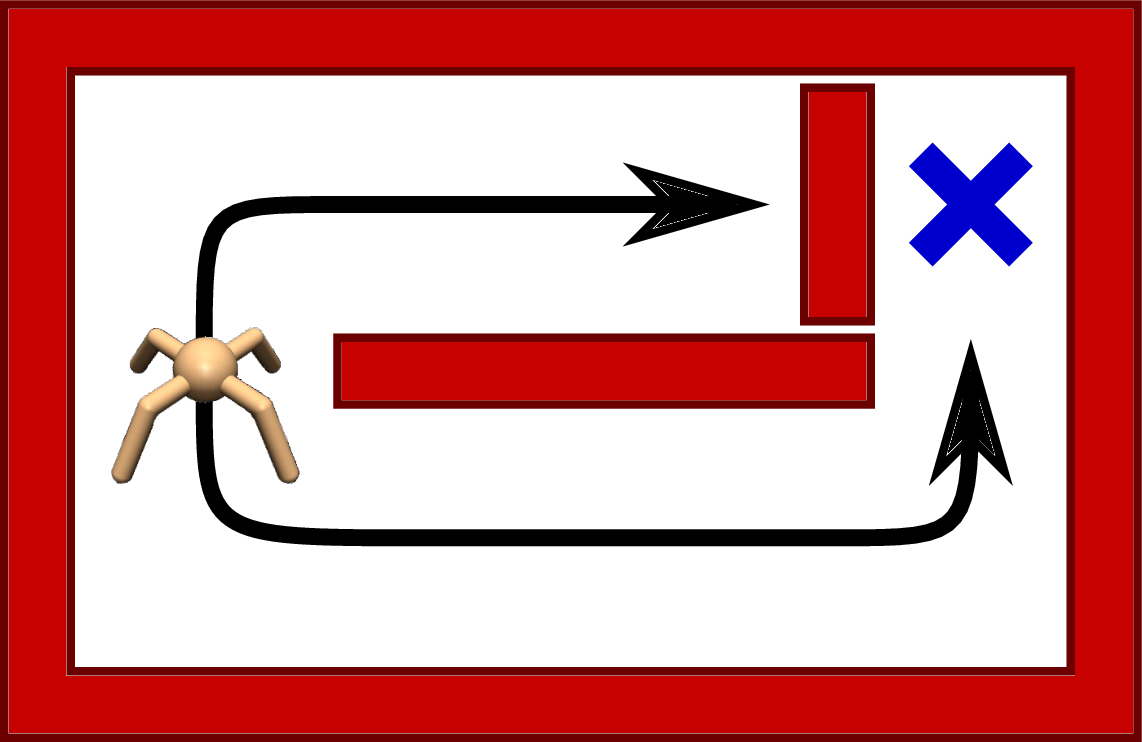
\includegraphics[width=\textwidth]{Images/twopaths.png}
\end{exampleBox}

Можно считать, что в данном фреймворке мы на самом деле лишь чуть-чуть модифицировали награду в среде:
\begin{equation}\label{softreward}
r_{\soft}(s, a) \coloneqq r(s, a) - \alpha \log \pi(a \mid s)
\end{equation}
Построенную теорию теперь нужно перепроверять, поскольку награда $r$ стала зависеть от параметров стратегии напрямую, да и очевидно, что не все утверждения переносятся на новую постановку:

\begin{proposition}
Оптимальной детерминированной стратегии может не существовать.
\begin{proof}
В MDP, где награда всегда 0, оптимальна стратегия с максимальной энтропией.
\end{proof}
\end{proposition}

Рассмотрим только нужные нам вещи. Будем обозначать оценочные функции в рамках данного фреймворка как $Q^\pi_{\soft}, V^\pi_{\soft}$. Также без ограничения общности далее будем считать $\alpha \HM= 1$, так как всегда можно перемасштабировать награду $r(s, a)$ без изменения задачи.

Мы также должны договориться о том, в какой момент во время взаимодействия приходит энтропийный бонус. Формула \eqref{softreward} предполагает, что после выбора действия $a$ из состояния $s$ помимо награды $r(s, a)$ агент ещё поощряется $\log \pi(a \mid s)$; однако мы договоримся по-другому\footnote{такая договорённость удобнее, поскольку после сэмплирования действия $a$ в состоянии $s$ неудобно учитывать зависимость награды от распределения $\pi(\cdot \HM\mid s)$.}. Будем считать, что агент, приходя в некоторое состояние $s$, получает бонус в размере $\entropy(\pi(\cdot \mid s)) \HM\coloneqq - \E_{a \sim \pi(a \mid s)} \log \pi(a \mid s)$ (если состояние не терминальное), затем сэмплирует действие $a$, получает бонус $r(s, a)$ и потом наблюдает $s'$. В такой договорённости уравнения для мягких оценочных функций выглядят так:

\begin{theorem}[Мягкие уравнения Беллмана (soft Bellman equations)]
$$Q^\pi_{\soft}(s, a) = r(s, a) + \gamma \E_{s'} V^\pi_{\soft}(s')$$
\begin{equation}\label{softVQ}
V^\pi_{\soft}(s) = \E_{\pi(a \mid s)} \left[ Q^\pi_{\soft}(s, a) - \log \pi(a \mid s) \right]
\end{equation}
\begin{proof}
По определению с учётом договорённости.
\end{proof}
\end{theorem}

\subsection{Вид оптимальной стратегии}

Как будет выглядеть критерий оптимальности Беллмана в задаче Maximum Entropy RL? По аналогии с обычным случаем, введём оптимальные оценочные функции:
$$V^*_{\soft}(s) \coloneqq \max_{\pi} V^{\pi}_{\soft}(s)$$
$$Q^*_{\soft}(s, a) \coloneqq \max_{\pi} Q^{\pi}_{\soft}(s, a)$$

\begin{theorem}
Оптимальной является стратегия
$$\pi(a \mid s) \propto \exp{Q^*_{\soft}(s, a)}$$
\beginproof[Доказательство] Проводим рассуждения аналогичные теореме \ref{th:nonstatbellmancriterion}. Откажемся от стационарности и будем рассматривать задачу поиска оптимальной стратегии $\pi_t(a \mid s_0)$ в предположении, что в будущем мы сможем набрать максимально возможную награду $Q^*_{\soft}(s, a, t)$:
$$\E_{\pi_t(a \mid s)} \left[ Q^*_{\soft}(s, a, t) - \log \pi_t(a \mid s) \right] \to \max\limits_{\pi_t(a \mid s)}
$$

Благодаря отказу от стационарности $Q^*_{\soft}(s, a_t, t)$ от $\pi_t$ не зависит. Чтобы решить эту задачу, заметим, что с точностью до константы, не зависящей от $\pi_t$, оптимизируемое выражение есть:
$$-\KL \left( \pi_t(a \mid s) \parallel \frac{\exp Q^*_{\soft}(s, a, t)}{Z(s, t)} \right) \to \max\limits_{\pi_t(a \HM\mid s)},$$
где $Z(s, t)$ --- нормировочная константа $\exp Q^*_{\soft}(s, a, t)$. Понятно, что оптимум достигается в нуле на $\pi_t(a \HM\mid s)$, совпадающей с этим распределением.

Дальнейшее рассуждение строится как раньше: $Q^*_{\soft}$ от времени не зависит по определению (аналогично утв. \ref{pr:nonstat_optimal_are_stat}), поэтому оптимальная стратегия получается стационарной, следовательно
\begin{equation*}
\pi(a \mid s) \propto \exp Q^*_{\soft}(s, a)   \tagqed
\end{equation*}
\end{theorem}

% Мы могли бы решать её и в лоб при помощи вычисления производной по Фреше. То есть: нам нужно решить задачу в функциональном пространстве для фиксированных $s, t$; вспомним, как в таком пространстве функций $\pi_t(\cdot \mid s)$ можно задать скалярное произведение:
% $$\langle f, g \rangle = \int\limits_\A f(a)g(a) \diff a$$
% Обозначим $Q(a) \coloneqq Q^*_{\soft}(s, \cdot, t)$, $\pi(a) \coloneqq \pi_t(\cdot \mid s)$. Тогда наша задача при фиксированных $s, t$ переписывается как:
% $$
% \begin{cases}
% \langle \pi(a), Q(a) \rangle - \langle \pi(a), \log \pi(a) \rangle \to \max\limits_{\pi(a)} \\
% \langle \pi(a), 1 \rangle = 1, \qquad \pi(a) \ge 0 
% \end{cases},
% $$
% где в равенстве 1 --- единичная функция (функция, которая для любого действия выдаёт 1).

% Решаем задачу: составляем лагранжиан (неравенство не учитываем, оптимальное решение удовлетворит ему автоматически).
% $$\mathcal{L}(\pi(a), \mu) = \langle \pi(a), Q(a) \rangle - \langle \pi(a), \log \pi(a) \rangle + \mu \langle \pi(a), 1 \rangle - \mu$$

% Дифференцируем (берём производную по Фреше) по $\pi$ и приравниваем к нулю, получаем
% $$\nabla_\pi \mathcal{L}(\pi, \mu) = Q(a) - \log \pi(a) - 1 + \mu = 0$$
% Итого:
% $$\log \pi_t(a \mid s) = Q^*_{\soft}(s, a, t) - 1 + \mu \quad \Rightarrow \quad \pi_t(a \mid s) \propto \exp Q^*_{\soft}(s, a, t)$$

Имея на руках вид оптимальной стратегии, мы можем получить уравнения оптимальности:

\begin{theorem}[Мягкие уравнения связи]
\begin{equation}\label{softV*Q*}
V^*_{\soft}(s) = \log \int\limits_{\A} \exp Q^*_{\soft}(s, a) \diff a
\end{equation}
\begin{proof}
Мы знаем, что оптимальная стратегия имеет вид $\pi(a \mid s) \HM= \frac{\exp{Q^*_{\soft}(s, a)}}{Z(s)}$, где
$$Z(s) \coloneqq \int\limits_{\A} \exp Q^*_{\soft}(s, a) \diff a$$
является нормировочной константой. Посчитаем энтропию такого распределения:
$$-\E_{\pi(a \mid s)} \log \pi(a \mid s) = \int\limits_{\A} \frac{\exp{Q^*_{\soft}(s, a)}}{Z(s)} \left(\log Z(s) - Q^*_{\soft}(s, a) \right) \diff a = \log Z(s) - \E_{\pi(a \mid s)} Q^*_{\soft}(s, a)$$

Подставим оптимальную стратегию в мягкое VQ уравнение \eqref{softVQ}:
\begin{align*}
V^\pi_{\soft}(s) &= \E_{\pi(a \mid s)} \left[ Q^\pi_{\soft}(s, a) - \log \pi(a \mid s) \right] = \\ &= \E_{\pi(a \mid s)} Q^*_{\soft}(s, a) - \E_{\pi(a \mid s)} Q^*_{\soft}(s, a) + \log Z(s) = \\ &= \log Z(s)
\end{align*}
Вспоминая определение $Z(s)$, получаем доказываемое.
\end{proof}
\end{theorem}

\begin{proposition}
$$Q^*_{\soft}(s, a) = r(s, a) + \gamma \E_{s'} V^*_{\soft}(s')$$
\end{proposition}

\begin{proposition}[Мягкое уравнение оптимальности Беллмана (soft Bellman optimality equations)]
\begin{equation}\label{softQ*Q*}
Q^*_{\soft}(s, a) = r(s, a) + \gamma \E_{s'} \log \int\limits_{\A} \exp Q^*_{\soft}(s', a') \diff a'
\end{equation}
\end{proposition}

\begin{theorem}
Оператор, стоящий в правой части уравнения \eqref{softQ*Q*}, является сжимающим с коэффициентом $\gamma$, и, следовательно, метод простой итерации решения этой системы уравнений сходится из любого начального приближения к единственной неподвижной точке.
\begin{proof}
Пусть даны две Q-функции, $Q_1, Q_2$, и пусть 
$$\rho(Q_1, Q_2) \coloneqq \max\limits_{s, a} | Q_1(s, a) \HM- Q_2(s, a) | \HM< \eps.$$
Тогда:
$$
\log \int\limits_{\A} \exp Q_1(s, a) \diff a \le \log \int\limits_{\A} \exp (Q_2(s, a) + \eps) \diff a = \eps + \log \int\limits_{\A} \exp Q_2(s, a) \diff a
$$
Аналогично можно показать, что 
$$
\log \int\limits_{\A} \exp Q_1(s, a) \diff a \ge -\eps + \log \int\limits_{\A} \exp Q_2(s, a) \diff a
$$

Пусть $\B_{\soft}$ --- оператор, стоящий в правой части \eqref{softQ*Q*}. Тогда:
\begin{align*}
| [\B_{\soft} Q_1](s, a) - [\B_{\soft} Q_2](s, a) | &= \gamma | \E_{s'} \left( \log \int\limits_{\A} \exp Q_1(s', a') \diff a' - \log \int\limits_{\A} \exp Q_2(s', a') \diff a' \right) | \le \\ 
&\le \gamma \eps
\end{align*}
Таким образом, $\rho(\B_{\soft} Q_1, \B_{\soft} Q_2)$ уменьшилось по крайней мере в $\gamma$ раз по сравнению с $\rho(Q_1, Q_2)$.
\end{proof}
\end{theorem}

\begin{proposition}
Если $\pi(a \mid s) \propto Q^{\pi}_{\soft}(s, a)$, то она оптимальна.
\begin{proof}
Q-функция такой стратегии удовлетворяет мягкому уравнению оптимальности Беллмана \eqref{softQ*Q*} и в силу единственности его решения совпадает с $Q^*_{\soft}(s, a)$.
\end{proof}
\end{proposition}

Итого, оптимальная стратегия имеет вид не аргмакса от Q-функции, а больцмановской стратегии \eqref{boltzman}. Мы теперь можем построить, например, аналог DQN для задачи Maximum Entropy RL, называемым \emph{Soft Q-learning}: для этого нужно заменить уравнение оптимальности Беллмана на мягкое уравнение оптимальности: таргет для перехода $\T \coloneqq (s, a, r, s')$ строить как
$$y(\T) \coloneqq r + \gamma \log \int\limits_{\A} \exp Q^*_{\soft}(s', a', \theta^{-}) \diff a',$$
где $\theta^{-}$ --- параметры таргет-сети. Интересно, что это соответствует <<учёту>> Больцмановской стратегии исследования внутри оценочной функции (нечто похожее мы делали в табличном алгоритме SARSA в разделе \ref{subsec:sarsa}). Однако, такой подход применим, как и в DQN, только для дискретных пространств действий, поскольку иначе стоящий в формуле интеграл мы аналитически не возьмём. Для непрерывных пространств действий нам нужно построить аналог DDPG.

\subsection{Soft Policy Improvement}

\begin{theoremBox}[label=th:softpi]{}
Пусть стратегии $\textcolor{ChadBlue}{\pi_1}$ и $\textcolor{ChadPurple}{\pi_2}$ таковы, что для всех состояний $s$ выполняется:
$$\E_{\textcolor{ChadPurple}{\pi_2}(a \mid s)} \textcolor{ChadBlue}{Q^{\pi_1}_{\soft}}(s, a) + \entropy(\textcolor{ChadPurple}{\pi_2}(\cdot \mid s)) \ge \textcolor{ChadBlue}{V^{\pi_1}_{\soft}}(s),$$
тогда $\textcolor{ChadPurple}{\pi_2} \succeq \textcolor{ChadBlue}{\pi_1}$ с учётом энтропийного бонуса; если хотя бы для одного $s$ неравенство выполнено строго, то $\textcolor{ChadPurple}{\pi_2} \succ \textcolor{ChadBlue}{\pi_1}$.
\begin{proof}
Полностью аналогично доказательству в обычном случае (теорема \ref{th:policyimprovement}).
\end{proof}
\end{theoremBox}

Если раньше для того, чтобы попасть под эту теорему, можно было взять $\textcolor{ChadBlue}{Q^{\pi_1}}(s, a)$ и взять от неё аргмакс по действиям, то теперь нужно промаксимизировать её по действиям с учётом добавки энтропийного бонуса. Мы уже поняли, что решением такой задачи будет больцмановская стратегия:

\begin{theorem}[Soft Policy Improvement]
Пусть $\textcolor{ChadBlue}{\pi_1}$ --- стратегия с мягкой оценочной функцией $\textcolor{ChadBlue}{Q^{\pi_1}_{\soft}}(s, a)$. Тогда стратегия $\textcolor{ChadPurple}{\pi_2}(a \mid s) \propto \exp \textcolor{ChadBlue}{Q^{\pi_1}_{\soft}}(s, a)$ не хуже $\textcolor{ChadBlue}{\pi_1}$.
\begin{proof}
Мы знаем, что такая $\textcolor{ChadPurple}{\pi_2}$ является решением задачи
$$\E_{\textcolor{ChadPurple}{\pi_2}(a \mid s)} \left[ \textcolor{ChadBlue}{Q^{\pi_1}_{\soft}}(s, a) - \log \textcolor{ChadPurple}{\pi_2}(a \mid s) \right] \to \max\limits_{\textcolor{ChadPurple}{\pi_2}(a \mid s)}
$$
Следовательно,
$$\E_{\textcolor{ChadPurple}{\pi_2}(a \mid s)} \textcolor{ChadBlue}{Q^{\pi_1}_{\soft}}(s, a) + \entropy(\textcolor{ChadPurple}{\pi_2}(\cdot \mid s)) \ge \E_{\textcolor{ChadBlue}{\pi_1}(a \mid s)} \textcolor{ChadBlue}{Q^{\pi_1}_{\soft}}(s, a) + \entropy(\textcolor{ChadBlue}{\pi_1}(\cdot \mid s)) = \textcolor{ChadBlue}{V^{\pi_1}_{\soft}}(s),$$
где последнее равенство следует из мягкого VQ уравнения \eqref{softVQ}. Значит, $\textcolor{ChadPurple}{\pi_2}$ попадает под теорему \ref{th:softpi}.
\end{proof}
\end{theorem}

Таким образом, Policy Iteration схема в задаче Maximum Entropy RL выглядит так:
\begin{itemize}
    \item \textbf{Policy Evaluation} заключается в обучении мягкой оценочной функции $Q^{\pi}_{\soft}(s, a)$ по данной стратегии $\pi$;
    \item \textbf{Policy Improvement} заключается в вычислении новой стратегии $\tilde{\pi}(\cdot \mid s) \propto \exp Q^{\pi}_{\soft}(s, a)$ по имеющейся оценочной функции;
\end{itemize}

\subsection{Обучение мягкого критика}

Итак, будем строить в рамках данного фреймворка Policy Iteration схему по аналогии с DDPG (алг. \ref{DDPGalgorithm}). Начнём с критика. Мы хотим решать мягкое уравнение Беллмана:
$$Q^\pi_{\soft}(s, a) \leftarrow r + \gamma \E_{s'} V_{\soft}^\pi(s') $$
где V-функция выражается через Q-функцию по формуле \eqref{softVQ}. Мы разделим это уравнение на два (не будем сводить к QQ-уравнению, как делали раньше) в силу того, что взять мат.ожидание по $\E_{a'}$ у нас не получится. Мы могли бы оценивать его Монте-Карло, но для уменьшения дисперсии в схеме предлагается завести третью сетку, которая будет учить $V^\pi_{\soft}(s, \psi)$: а именно, учить мат.ожидание $\E_{a'}$, опять же, через сведение к задаче регрессии:
$$V_{\soft}^\pi(s) \leftarrow \E_{a} \left[ Q^\pi_{\soft}(s, a) - \log \pi(a \mid s) \right]$$

Таким образом, таргеты для критика (Q-функция с параметрами $\omega$) и для вспомогательной V-функции выглядят так: для заданного перехода $\T \HM= (s, a, r, s')$, взятого из буфера, генерируем $\hat{a}$ из текущей версии стратегии $\pi$ и запоминаем вероятность $\pi(\hat{a} \HM\mid s)$, после чего вычисляем таргеты по следующим формулам:
$$y_Q(\T) \coloneqq r + \gamma V^\pi_{\soft}(s', \psi)$$
$$y_V(\T) \coloneqq Q^\pi_{\soft}(s, \hat{a}, \omega) - \log \pi(\hat{a} \mid s)$$
И с такими таргетами, как обычно, решаем задачу регрессии с функцией потерь MSE. Самое главное --- соответствующее действие $\hat{a}$ для таргета $y_V$ брать не из буфера, а сгенерировать из текущей версии стратегии, поскольку иначе мы сдвинемся в сторону V-функции не текущей стратегии $\pi$, а той стратегии, которая выбирала $a$ из буфера.

Для стабилизации процесса предлагаются следующие эвристики\footnote{в DDPG-подобных схемах дать однозначный ответ, где нужно использовать таргет-сеть, а где нет, сложно. Понятно лишь то, что для стабилизации какие-то эвристики необходимы; без таргет-сетей эти алгоритмы не заработают. В этих моментах могут различаться и реализации алгоритмов.}: завести таргет-сеть (с параметрами $\psi^{-}$) для V-функции и использовать её при построении таргета $y_Q$ для Q-функции:
$$y_Q(\T) \coloneqq r + \gamma V^\pi_{\soft}(s', \psi^{-}),$$
а для борьбы с overestimation bias в таргете для V-функции использовать clipped double оценку (раздел \ref{subsec:clippedtwin}), то есть учить две Q-функции с параметрами $\omega_1, \omega_2$ и строить таргет $y_V$ по следующей формуле: 
$$y_V(\T) \coloneqq \min_{i = {1, 2}} Q^\pi_{\soft}(s, \hat{a}, \omega_i) - \log \pi(a \mid s)$$

\subsection{Обучение мягкого актёра}

Для обучения актёра мы теперь хотим не максимизировать Q-функцию по действиям, а выучить распределение $\pi_\theta(a \HM\mid s) \HM\propto \exp{Q^\pi_{\soft}(s, a, \omega)}$. Для этого будем просто минимизировать, например, $\KL$-дивергенцию между этими двумя распределениями по параметрам стратегии $\theta$. Предлагается взять такую:
$$\KL(\pi_\theta(a \mid s) \parallel \exp Q^\pi_{\soft}(s, a)) \to \min_\theta$$

Мы опять же делаем это как бы одновременно для всех состояний, поэтому откуда будем брать состояния --- не принципиально, сгодится из буфера. Таким образом схема, как и в DDPG, получится off-policy. Проблем с минимизацией KL-дивергенции не возникает:

\begin{theorem}
$$\KL(\pi_\theta(a \mid s) \parallel \exp Q^\pi_{\soft}(s, a)) = \E_{a \sim \pi_\theta(a \mid s)} \left[ \log \pi_\theta(a \mid s) - Q^\pi_{\soft}(s, a) \right] + \const(\theta)$$
\beginproof
По определению, с единственной оговоркой, что у распределения $\exp Q^\pi_{\soft}(s, a)$ есть некоторая нормировочная константа $Z(s) \coloneqq \int\limits_\A \exp Q^\pi_{\soft}(s, a) \diff a$, но слагаемое
\begin{equation*}
\E_{a \sim \pi_\theta(a \mid s)} \log Z(s) = \log Z(s) = \const(\theta)    \tagqed
\end{equation*}
\end{theorem}

Итак, функционал для оптимизации актёра выглядит так (заменяя минимизацию на максимизацию):
\begin{equation}\label{stochactor}
\E_{a \sim \pi_\theta(a \mid s)} \left[ -\log \pi_\theta(a \mid s) + Q^\pi_{\soft}(s, a) \right] \to \max_{\theta}
\end{equation}

Первое слагаемое --- энтропию $\pi_\theta(a \mid s)$ --- обычно можно рассчитать для выбранной параметризации $\pi_{\theta}(a \HM\mid s)$. Рассмотрим второе слагаемое (среднее Q-функции по действиям); тут возможно два случая. Допустим, стратегия выдаёт распределение, для которого работает \emph{репараметризационный трюк} (reparameterization trick): а то есть, если сэмплирование $a \HM\sim \pi_\theta(a \mid s)$ эквивалентно сэмплированию шума из некоторого не зависящего от параметров распределения $\eps \sim p(\eps)$ и его дальнейшего детерминированного преобразования $a \HM= \pi_{\theta}(s, \eps)$. Тогда второе слагаемое в \eqref{stochactor} мы сможем оптимизировать по $\theta$ через этот репараметризационный трюк:
\begin{equation*}
\E_{a \sim \pi_\theta(a \mid s)} Q^\pi_{\soft}(s, a) = \E_{\eps \sim p(\eps)} Q^\pi_{\soft}(s, \pi_{\theta}(s, \eps))
\end{equation*}
Теперь стохастическая оценка градиента по $\theta$ получается напрямую. Понятно, что мы получили обобщение формулы \eqref{ddpg_actor}; мы оптимизируем актёра при помощи градиентов из критика, но дополнительно впрыскиваем шум в действия для получения стохастичной стратегии, а также добавляем энтропийное слагаемое. 

\begin{exampleBox}[label=ex:gaussianactor_sac]{}
Пусть наша стратегия параметризована нормальным распределением $\pi_\theta(a \mid s) \HM\coloneqq \N(\mu(s, \theta), \sigma(s, \theta)^2I)$. Для неё можно проводить репараметризационный трюк: сэмплирование действий эквивалентно $a \coloneqq \mu(s, \theta) \HM+ \eps \HM\odot \sigma(s, \theta)$, где $\eps \HM\sim \N(0, I)$, $\odot$ --- поэлементное перемножение. Для него также можно аналитически посчитать энтропию:
$$\entropy(\N(\mu, \sigma^2I)) = \sum_{i=1}^{A} \log \sigma_i$$

Итого, формула \eqref{stochactor} в таком случае получается следующей:
$$\sum_{i=1}^A\log \sigma_i(s, \theta) + \E_{\eps \sim \N(0, I)} Q^\pi_{\soft}(s, \mu(s, \theta) + \sigma(s, \theta) \eps) \to \max_\theta $$
\end{exampleBox}

Мы, однако, можем захотеть выбрать более сложную параметризацию стратегии, для которой не применим репараметризационный трюк и нельзя аналитически посчитать энтропию. Тогда нам придётся при взятии градиента в \eqref{stochactor} применить оценку в стиле REINFORCE:

\begin{proposition}
Градиент \eqref{stochactor} равен
$$\nabla_\theta = \E_{a \sim \pi_\theta(a \mid s)} \nabla_{\theta} \log \pi_\theta(a \mid s) \left[ -\log \pi_\theta(a \mid s) + Q^\pi_{\soft}(s, a) - b(s) \right],$$
где $b(s)$ --- бэйзлайн, произвольная функция от состояний.
\end{proposition}

Как и в policy gradient подходе, разумным бэйзлайном является среднее по действиям величины $b(s) \coloneqq \E_a -\log \pi_\theta(a \mid s) + Q^\pi_{\soft}(s, a) = V^\pi_{\soft}(s)$. Мы как раз учим вспомогательную V-функцию при обучении критика, и как раз можем этой оценкой воспользоваться для сбивания дисперсии. Таким образом, формула градиента принимает вид
$$\nabla_\theta = \E_{a \sim \pi_\theta(a \mid s)} \log \pi_\theta(a \mid s) \left[ -\log \pi_\theta(a \mid s) + Q^\pi_{\soft}(s, a) - V^\pi_{\soft}(s) \right]$$

\begin{example}
Этой формулой понадобится пользоваться, например, если актёр моделирует распределение в виде смеси гауссиан. Преимущество смеси перед одной гауссианой --- многомодальность. Тогда при использовании $K$ компонент смеси актёр для данного состояния $s$ выдаёт следующие величины: $K$ суммирующихся в единицу чисел $w_i(s, \theta)$, а также $K$ векторов $\mu_i(s, \theta), \sigma_i(s, \theta)$, где $i \in {1, 2, \dots, K}$. Итоговое распределение полагается
$$\pi_\theta(a \mid s) \coloneqq \sum_{i = 1}^K w_i(s, \theta) \N(\mu_i(s, \theta), \sigma_i(s, \theta)^2I)$$
\end{example}

\subsection{Soft Actor-Critic (SAC)}

Далее схема приведена для простоты для случая, если актёр моделирует гауссиану (см. пример \ref{ex:gaussianactor_sac}). 

\begin{algorithm}[label = SACalgorithm]{Soft Actor-Critic (SAC)}
\textbf{Гиперпараметры:} $B$ --- размер мини-батчей, $\tau$ --- параметр экспоненциального сглаживания таргет-сети, $\pi_{\theta}(a \mid s) \coloneqq \N(\mu_{\theta}(s), \sigma_{\theta}(s)^2 I)$ --- гауссова стратегия с параметрами $\theta$, $Q^\pi_{\soft}(s, a, \omega_i)$ --- две нейросетки с параметрами $\omega_1$ и $\omega_2$, $V^\pi_{\soft}(s, \psi)$ --- нейросетка с параметрами $\psi$, SGD-оптимизаторы.

\vspace{0.3cm}
Инициализировать $\theta, \omega_1, \omega_2, \psi$ произвольно \\
Положить $\psi^- \coloneqq \psi$ \\
Пронаблюдать $s_0$ \\
\textbf{На очередном шаге $t$:}
\begin{enumerate}
    \item выбрать $a_t \sim \pi_\theta(a_t \mid s_t)$
    \item пронаблюдать $r_t$,  $s_{t+1}$, $\done_{t+1}$
    \item добавить пятёрку $(s_t, a_t, r_t, s_{t+1}, \done_{t+1})$ в реплей буфер
    \item засэмплировать мини-батч размера $B$ из буфера
    \item для каждого $s$ из батча засэмплировать шума $\eps(s) \sim \N(0, I)$ и посчитать $\mu(s, \theta)$, $\sigma(s, \theta)$ стратегии $\pi_\theta$
    \item посчитать оценку градиента по параметрам стратегии:
    $$\nabla_\theta \coloneqq \frac{1}{B}\sum_{s \in B} \nabla_\theta \left[ \sum_{i=0}^A \log \sigma_i(s, \theta) + Q^\pi_{\soft}(s, \mu(s, \theta) + \sigma(s, \theta) \eps(s), \omega_1) \right]$$
    \item делаем шаг градиентного подъёма по $\theta$, используя $\nabla_\theta$
    \item для каждого перехода $\T \coloneqq (s, a, r, s', \done)$ засэмплировать $a' \sim \pi_\theta(a' \mid s')$ и сохранить вероятности $\pi_\theta(a' \mid s')$
    \item посчитать таргеты:
    $$y_V(\T ) \coloneqq \min_{i = 1, 2} Q^\pi_{\soft}\left( s', a', \omega_i \right) - \log \pi_\theta(a' \mid s')$$
    $$y_Q(\T ) \coloneqq r + \gamma V^\pi_{\soft}\left( s', \psi^{-} \right)$$
    \item посчитать лоссы:
    $$\Loss_V(\psi) \coloneqq \frac{1}{B}\sum_{\T} \left( V^\pi_{\soft}(s', \psi) - y_V(\T ) \right) ^2$$
    $$\Loss_{Q1}(\omega_1) \coloneqq \frac{1}{B}\sum_{\T} \left( Q^\pi_{\soft}(s, a, \omega_1) - y_Q(\T ) \right) ^2$$
    $$\Loss_{Q2}(\omega_2) \coloneqq \frac{1}{B}\sum_{\T} \left( Q^\pi_{\soft}(s, a, \omega_2) - y_Q(\T ) \right) ^2$$
    \item делаем шаг градиентного спуска по $\psi$, $\omega_1$ и $\omega_2$, используя $\nabla_\psi \Loss_V(\psi)$, $\nabla_\omega \Loss_{Q1}(\omega_1)$ и $\nabla_{\omega_2} \Loss_{Q2}(\omega_2)$ соответственно
    \item обновляем таргет-сеть: $\psi^{-} \leftarrow \tau \psi^{-} + (1 - \tau) \psi$
\end{enumerate}
\end{algorithm}
